\newpage
\section{Integration (bi-variat)}
Als bi-variate Integrale versteht man Integrale, die siech über zwei unabhängige Variablen erstrecken.
Sie haben die Form
\[
    \int\limits_{\Omega} f(\omega)\cdot \diff \omega =\int\limits_{X} \int\limits_{Y} f(x;y) \cdot dy \cdot dx
\]
wobei $ \Omega \subset \mathbb{R}^2 $, $ X \subset \mathbb{R} $ und $ Y \subset \mathbb{R} $ ist.

\subsection{Normalbereich}

TODO: WTF ist ein Normalbereich?
Schnitte sind Strecken (Intervalle) für x, y, ...

\subsection{Zweidimensionale Koordinatensysteme}
Neben den Kartesischen Koordinatensystemen kommen in zweidimensionalen Räumen auch Polare Koordinatensysteme zum Einsatz.
Die beiden Systeme können mit Hilfe der Trigonometrie in einander überführt werden.

\subsubsection{Umrechnung Kartesisch $\leftrightarrow$ Polar}
\begin{minipage}{0.29\linewidth}
    \myul{Polar zu Kartesisch}
    \[
    \begin{pmatrix}
        x \\
        y
    \end{pmatrix}
    =
    \begin{pmatrix}
        r * \cos{\varphi}\\
        r * \sin{\varphi}
    \end{pmatrix}
    \]
\end{minipage}
\hfill
\begin{minipage}{0.29\linewidth}
    \myul{Kartesisch zu Polar}
    \[
    \begin{pmatrix}
        r \\
        \varphi
    \end{pmatrix}
    =
    \begin{pmatrix}
        \sqrt{x^2+y^2}\\
        \tan^{-1}{\frac{y}{x}}
    \end{pmatrix}
    \]
\end{minipage}
\hfill
\begin{minipage}{0.29\linewidth}
    \begin{center}
        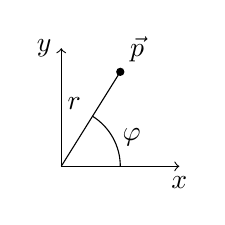
\begin{tikzpicture} [scale = 1.5]
            % Kartesische Achsen
            \draw[->] (0, 0) -- (1, 0) node [below] {$x$} ;
            \draw[->] (0, 0) -- (0, 1) node [left]  {$y$} ;

            % Punkt p
            \fill (0.5, 0.8) circle (1pt) node [anchor=south west] {$\vec{p}$};

            % Länge r
            \draw (0, 0) -- (0.5, 0.8) node [midway, above left] {$r$};
            % Winkel phi
            \draw (0.5, 0) arc (0:58:0.5) node [midway, right] {$\varphi$};
        \end{tikzpicture}
    \end{center}
\end{minipage}

Dabei ist zu beachten, dass $\tan^{-1}$ nur werte von $-180\degree$ bis $180\degree$ liefert. 
$\varphi$ wird also, je nach dem in welchem Quadranten sich $\vec{p}$ befindet, nach folgendem Schema berechnet:
\begin{center}
    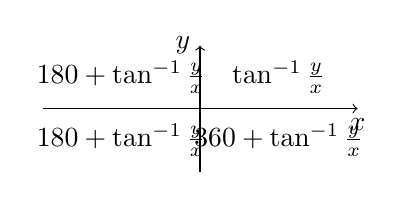
\begin{tikzpicture}
        % Achsen 
        \draw [->] (-2, 0) -- (2, 0) node [below] {$x$};
        \draw [->] (0, -0.8) -- (0, 0.8) node [left] {$y$};
        % Formeln
        \node at ( 1,  0.4) {$\tan^{-1}\frac{y}{x}$};
        \node at ( 1, -0.4) {$360\degree + \tan^{-1}\frac{y}{x}$};
        \node at (-1, -0.4) {$180\degree + \tan^{-1}\frac{y}{x}$};
        \node at (-1,  0.4) {$180\degree + \tan^{-1}\frac{y}{x}$};
    \end{tikzpicture}
\end{center}

Um eine ganzes Integral vom einen Koordinatensystem ins andere zu überführen, muss zum einen die Funktion $ f(x, y) $ zu $ f(r, \varphi) $ (oder umgekehrt) umgeschrieben, sowie die differentiale angepasst werden.
Hier dafür einige gängige Elemente:

\begin{tabular}{l c c}
                         & \bf{Kartesisch}                   & \bf{Polar}                                                       \\
    \bf{x-Achsenelement} & $\diff x$                         & $\diff x = \cos \varphi \diff r - r \sin \varphi \diff \varphi$  \\
    \bf{y-Achsenelement} & $\diff y$                         & $\diff x = \sin \varphi \diff r + r \cos \varphi \diff \varphi$  \\
    \bf{Linienelement  } & $\diff s^2 = \diff x^2 \diff y^2$ & $\diff s^2 = \diff r^2 + r^2 \diff \varphi^2$                    \\
    \bf{Flächenelement } & $\diff A = \diff x \diff y$       & $\diff A = r \diff r \diff \varphi$                              \\
\end{tabular}

\subsection{2D Transformation Polar zu Kartesisch}
TODO: Das isch ja ds gliiche wie obe beschribe, oder?
      Wänn da no meh ane sött wüsstich nöd was... -Flurin
T $=$ Transformation
\[
    \text{Polar } (r,\varphi) \xrightarrow{T} (x,y) \text{ Kartesisch}
\]

\[
\begin{pmatrix}
    x=r\cdot\cos(\varphi) \text{ } \cor{\mathbb{R}} \\
    y=r\cdot\sin(\varphi) \text{ } \cor{\mathbb{R}} 
\end{pmatrix}
\text{2D}
\]

Die Funktionen für $x$ und $y$ sind skalare Funktion.

    \begin{ctabular}{ll}
        $x=x(r;\varphi)$ & $ y=y(r;\varphi)$
    \end{ctabular}

\subsection{Derivative, Ableitung}
TODO: Idk was da ane söll -Flurin

\subsection{Anwendungsformeln Doppelintegral}
\resizebox{\linewidth}{!}{
    \begin{tabular}{|l|l|l|}
        \hline
        \bf{Allgemein} & \bf{Kartesische Koordinaten} & \bf{Polarkoordinaten} \\
        \hline

        \multicolumn{3}{|l|}{\bf{Flächeninhalt einer ebenen Figur}} \\\hline
        $ A = \int\limits_{A} \diff a $ & 
        $ = \int\limits_{X}\int\limits_{Y} \diff y \diff x $ &
        $ = \int\limits_{\Phi}\int\limits_{R} r \diff r \diff \varphi $ \\\hline

        \multicolumn{3}{|l|}{\bf{Oberfläche einer Ebene in drei Dimensionen}} \\\hline
        % TODO: Ka, ob das stimmt, evtl. umschreiben, dass man es besser versteht...
        % Ist aus Bernies unterlagen abgeschrieben.
        $ S = \int\limits_{A} \frac{1}{\cos \gamma} \diff a $ & 
        $ = \int\limits_{X}\int\limits_{Y} \sqrt{1 + \left(\frac{\partial z}{\partial x}\right)^2 + \left(\frac{\partial z}{\partial y}\right)^2} \diff y \diff x $ &
        $ = \int\limits_{\Phi}\int\limits_{R} \sqrt{r^2 + r^2\left(\frac{\partial z}{\partial r}\right)^2 + \left(\frac{\partial z}{\partial \varphi}\right)^2} \diff r \diff \varphi $ \\\hline
        
        \multicolumn{3}{|l|}{\bf{Volumen eines Zylinders}} \\\hline
        $ V = \int\limits_{A} z \diff a $ & 
        $ = \int\limits_{X}\int\limits_{Y} z \diff y \diff x $ &
        $ = \int\limits_{\Phi}\int\limits_{R} z r \diff r \diff \varphi $ \\\hline

        \multicolumn{3}{|l|}{\bf{Trägheitsmoment einer ebenen Figur, bezogen auf die x-Achse}} \\\hline
        $ I_x = \int\limits_{A} y^2 \diff a $ & 
        $ = \int\limits_{X}\int\limits_{Y} y^2 \diff y \diff x $ &
        $ = \int\limits_{\Phi}\int\limits_{R} r^3 \sin^2\varphi \diff r \diff \varphi $ \\\hline

        \multicolumn{3}{|l|}{\bf{Trägheitsmoment einer ebenen Figur, bezogen auf den Pol $(0, 0)$}} \\\hline
        % TODO: wieso r^3? evtl. nachrechnen, scheint iwie komisch...
        $ I_x = \int\limits_{A} r^2 \diff a $ & 
        $ = \int\limits_{X}\int\limits_{Y} (x^2 + y^2) \diff y \diff x $ &
        $ = \int\limits_{\Phi}\int\limits_{R} r^3 \diff r \diff \varphi $ \\\hline

        \multicolumn{3}{|l|}{\bf{Masse einer ebenen Figur mit Dichtefunktion $\varrho$}} \\\hline
        $ m = \int\limits_{A} \varrho \diff a $ & 
        $ = \int\limits_{X}\int\limits_{Y} \varrho (x, y) \diff y \diff x $ &
        $ = \int\limits_{\Phi}\int\limits_{R} \varrho (x, y) r \diff r \diff \varphi $ \\\hline

        \multicolumn{3}{|l|}{\bf{Koordinaten des Schwerpunkts einer homogenen, ebenen Figur}} \\\hline
        $ x_{COG} = \frac{\int\limits_{A} x \diff a}{A} $ & 
        $ = \frac{\int\limits_{X}\int\limits_{Y} x \diff y \diff x}{\int\limits_{X}\int\limits_{Y} \diff y \diff x} $ &
        $ = \frac{\int\limits_{\Phi}\int\limits_{R} r^2 \cos \varphi \diff r \diff \varphi}{\int\limits_{\Phi}\int\limits_{R} r \diff r \diff \varphi} $ \\
        $ y_{COG} = \frac{\int\limits_{A} y \diff a}{A} $ & 
        $ = \frac{\int\limits_{X}\int\limits_{Y} y \diff y \diff x}{\int\limits_{X}\int\limits_{Y} \diff y \diff x} $ &
        $ = \frac{\int\limits_{\Phi}\int\limits_{R} r^2 \sin \varphi \diff r \diff \varphi}{\int\limits_{\Phi}\int\limits_{R} r \diff r \diff \varphi} $ \\\hline
    \end{tabular}
}
\smallskip
